%\chapter{操作系统内核构建概述}
%\section{什么是操作系统}
%\subsection{体系结构}

\section{Busybox简介}
\subsection{简单介绍}

\begin{table}[h!]
	\begin{center}
		\caption{Busybox源码目录结构}
		\begin{tabular}{c|c|c} % <-- Alignments: 1st column left, 2nd middle and 3rd right, with vertical lines in between
			\textbf{序号} & \textbf{目录名称} & \textbf{功能说明}\\
			\hline
			1 & applets & 实现applets框架的文件,目录中包含了几个main0的文件。\\
			2 & applets sh & 此目录包含了几个作为shel脚本实现的applet示例。\\
			3 & arch & 包含用于不同体系架构的makefile文件。\\
			4 & archival & 与压缩相关命令的实现源文件。\\
			5 & configs & Busybox自带的默认配置文件。\\
			6 & console-tools & 与控制台相关的一些命令。\\
			7 & coreutils & 常用的一些核心命令。例如chgrp、m等。\\
			8 & debianutils & 针对Debian的套件。\\
			9 & e2fsprogs & 针对Linux Ext2 FS prog的命令,例chattr、 Isattr。\\
			10 & editors & 常用的编辑命令,例如diff、vi等。\\
			11 & findutils sh & 用于查找的命令。\\
			12 & include & Busybox项目的头文件。\\
			13 & init & init进程的实现源码目录。\\
			14 & klibc-utils & klibc命令套件。\\
			15 & libbb & 与Busybox实现相关的库文件。\\
			16 & libpwdgrp & libpwdgrp相关的命令。\\
			17 & loginutils & 与用户管理相关的命令。\\
			18 & mailutils & 与mail相关的命令套件。\\
			19 & miscutils & 该文件下是一些杂项命令,针对特定应用场景。\\
			20 & modutils & 与模块相关的命令。\\
			21 & networking & 与网络相关的命令,例arp。\\
			22 & printutils & Print相关的命令。\\
			23 & procps & 与内存、进程相关的命令。\\
			24 & runit & 与Runit实现相关的命令。\\
			25 & shell & 与shell相关的命令。\\
			26 & sysklogd & 系统日志记录工具相关的命令。\\
			27 & util-inux & Linux下常用的命令,主要与文件系统操作相关的命令。\\
		\end{tabular}
	\end{center}
\end{table}


Busybox是一个针对嵌入式系统的轻量级工具集合,旨在通过整合常用的
Linux命令和服务程序,将它们合并为一个单一的可执行文件。这个项目
最初于1996年诞生,当时嵌入式系统并不像今天这般普及。Busybox的
最初目的是为软盘系统设计的,因为在那个时候,可移动存储介质的容
量十分有限,软盘是主要的存储媒介之一。

Busybox的设计理念非常巧妙。相较于单独存放每个命令所需的存储空间
,Busybox通过将不同命令的共享部分整合到一起,极大地减小了可执行
文件的体积。举例来说,诸如grep和find这样的命令,尽管功能有所差
异,但它们都需要从文件系统中搜索文件,Busybox将这部分代码进行
共享,从而节省了空间。

Busybox的核心特点在于其高度紧凑的特性。它可以包含最基本的系统
命令,例如文件列表显示命令ls和文件内容查看命令cat,同时也能整
合更复杂的程序,如文本搜索命令grep和文件查找命令find,甚至还
能将HTTP服务器整合进同一个软件包中。

对于嵌入式系统来说,存储空间十分宝贵,而Busybox的存在则为这些
系统提供了解决方案。通常情况下,Busybox的可执行文件大小仅约1MB
左右,相比于分散存放各个命令所需的存储空间,这是一个相当节省空间
的选择。用户可以通过建立链接的方式,与传统的命令一样使用Busybox
,只不过它将多个功能整合到一个文件中,从而在嵌入式系统中占用更少
的存储空间。

Busybox源码目录结构图如上,方便以后对Busybox做裁剪的时候参考。

\subsection{工作原理}
Busybox利用了shell传递给C语言main()函数的参数,回想一下C语言
main()函数的定义:int main(int argc,char *argv[])

在main()函数的定义中argc是传递进来的参数个数,argv是一个字符串
数组,数据的每一项都是一个参数内容。其中,argv[0]是从命令行调用
的程序名。下面是一个简单的程序,使用argv[0]确定调用来自哪个程序
。

\begin{lstlisting}[language=Rust]
	//test.c
	#include <stdio.h>
	/*定义主函数*/
	int main(int argc,char *argv[])
	int i;
	for(i=0;i<argc ;i++){
		//for循环语句
		printf("argv[%d]=%s\n",i,argv[i]);//打印程序参数内容
	}
	return 0;
}
\end{lstlisting}

调用这个程序会显示所调用的第一个参数是该程序的名字。可以对这个可执行程序重新进行命名,此时再调用就会得到该程序的新名字。另外,可以创建一个到可执行程序的符号链接,在执行这个符号链接时,就可以看到这个符号链接的名字。

\begin{lstlisting}[language=Rust]
$  gcc -Wall -o test test.c
$  ./test argl arg2
argv[0]=./test
argv[1]=arg1
argv[2]=arg2

$  mv test newtest
$  ./newtest argl
argv[0]=./newtest
argv[1]=arg1

$  ln -s newtest linktest
$  ./linktest arg
argv[0]=./linktest
argv[1]=arg
\end{lstlisting}

Busybox使用符号链接屏蔽了程序调用细节。从用户的角度看,使用Busybox与使用传统的命令效果是相同的。Busybox为其包含的每个系统程序都建立了类似的符号链接。当用户使用符号链接调用Busybox的时候,Busybox通过argv[0]参数调用对应的功能函数。

\subsection{使用方法}
Busybox 的编译过程与Linux内核的编译类似。

Busybox的使用有三种方式:

Busybox后直接跟命令,如 Busybox ls。

直接将Busybox重命名,如 cp Busybox tar。

创建符号链接,如 ln -s Busybox rm。

以上方法中,第三种方法最方便,但为Busybox中每个命令都创建一个软链接,相当费事,Busybox提供自动方法:Busybox编译成功后,执行make install,则会产生一个\_install目录,其中包含了Busybox及每个命令的软链接
Busybox的使用方法与传统的Unix工具类似,通常的语法格式为:
Busybox [选项] [命令] [参数]。

Busybox的命令和参数根据具体的工具而定,可以通过以下方式获取帮助信息:
Busybox --help

\subsubsection{Busybox安装}
首先进入Busybox官网https://www.busybox.net/,选择所需版本下载。

\begin{figure}[H]
\centering
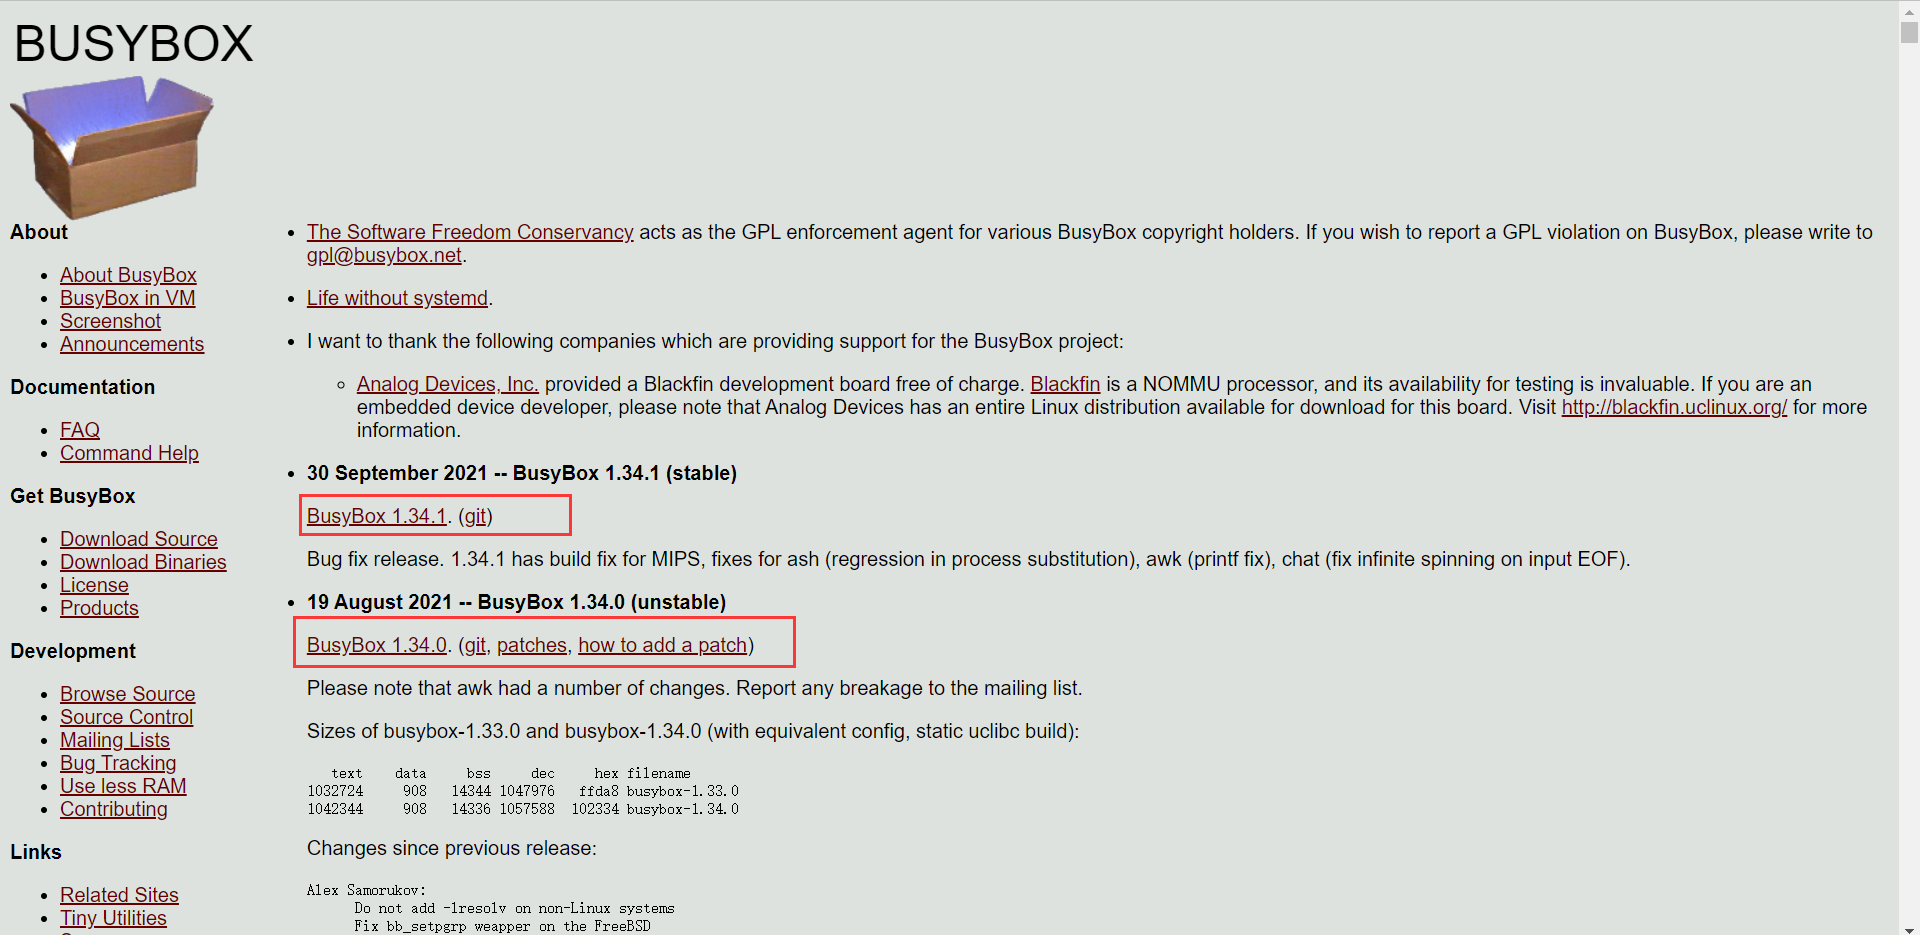
\includegraphics[width=17cm,height=10cm]{figures/09-02-Busybox安装1.png}
\caption{09-02-Busybox官网界面}
\end{figure}  

接下来将右击解压也可以使用命令行解压。

\begin{figure}[H]
\centering
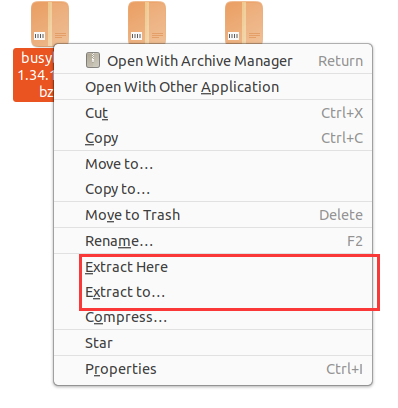
\includegraphics[width=10cm,height=6cm]{figures/09-02-Busybox安装2.png}
\caption{Busybox安装包解压}
\end{figure}  

进入解压后的目录

\begin{lstlisting}[language=Rust]
make defconfig  //使用默认配置,让Busybox包含常用命令和工具
make menuconfig  //在上述基础上,自己更改配置
\end{lstlisting}

\begin{figure}[H]
\centering
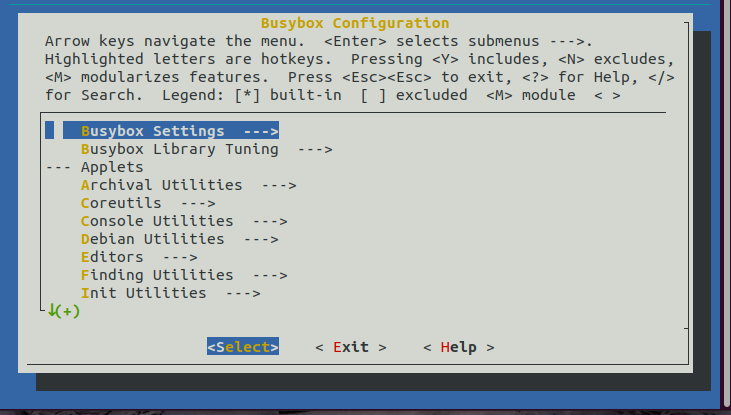
\includegraphics[width=14cm,height=8cm]{figures/09-02-Busybox安装3.png}
\caption{Busybox配置界面}
\end{figure}  

BusyBox Setting->Build Options->[ 选]Build Busybox as a static binary (no shared libs)

Shells->chose your default shell(ash):

BusyBox Setting->[*]Don’t use/usr(否则Busybox会安装到ubuntu的/usr下,会覆盖原系统原有的命令)

Coreutils—>sync

Linux System Utilities—>nsenter

Linux System Utilities—>Support mounting NFS filesystems(网络文件系统)

Networking Utilities—>inetd(超级服务器)

Busybox settings ->build options ->build with large file support

编译和安装Busybox

\begin{lstlisting}[language=Rust]
make
make install
\end{lstlisting}

当出现下图所示时就表明已经安装完成了。

\begin{figure}[H]
\centering
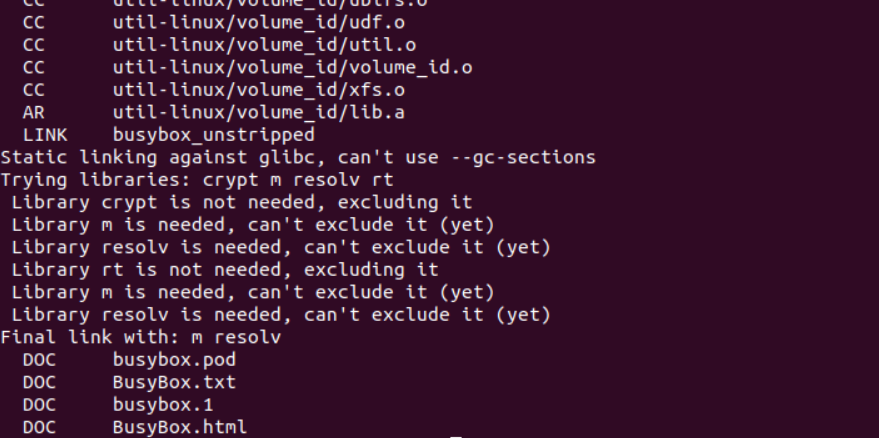
\includegraphics[width=14cm,height=8cm]{figures/09-02-Busybox安装4.png}
\caption{Busybox安装成功}
\end{figure}  

执行完成后会发现多了一个\_install目录。

\subsection{常用的命令}
\subsubsection{安装和登录命令}
\textbf{reboot:}

作用:reboot命令的作用是重新启动计算机,它的使用权限是系统管理者。

格式:reboot [-n] [-w] [-d] [-f] [-i]

主要参数:

-n: 在重开机前不做将记忆体资料写回硬盘的动作。

-w: 并不会真的重开机,只是把记录写到/var/log/wtmp文件里。

-d: 不把记录写到/var/log/wtmp文件里(-n这个参数包含了-d)。

-i: 在重开机之前先把所有与网络相关的装置停止。

\textbf{mount:}

作用:mount命令的作用是加载文件系统,它的用权限是超级用户或/etc/fstab中允许的使用者。

格式:mount -a [-fv] [-t vfstype] [-n] [-rw][-F] device dir

主要参数:

-v:显示信息,通常和-f用来除错。

-a:将/etc/fstab中定义的所有文件系统挂上。

-F:这个命令通常和-a一起使用,它会为每一个mount的动作产生一个行程负责执行。在系统需要挂上大量NFS文件系统时可以加快加载的速度。

\textbf{exit:}

作用:exit命令的作用是退出系统,它的使用权限是所有用户。

格式:exit

\subsubsection{文件处理命令}

\textbf{mkdir:}

作用:mkdir命令的作用是建立名称为dirname的子目录,与MS DOS下的md命令类似,它的使用权限是所有用户。

格式:mkdir [options] 目录名

主要参数:

-m, --mode=模式:设定权限,与chmod类似。

-p, --parents:需要时创建上层目录;如果目录早已存在,则不当作错误。

-v, --verbose:每次创建新目录都显示信息。

\textbf{grep:}

作用:grep命令可以指定文件中搜索特定的内容,并将含有这些内容的行标准输出。grep全称是Global Regular ExpressionPrint,表示全局正则表达式版本,它的使用权限是所有用户。

格式:grep [options]

主要参数:

-c:只输出匹配行的计数。

-I:不区分大小写(只适用于单字符)。

-h:查询多文件时不显示文件名。

\textbf{find:}

作用:find命令的作用是在目录中搜索文件,它的使用权限是所有用户。

格式:find [path][options][expression]

path指定目录路径,系统从这里开始沿着目录树向下查找文件。它是一个路径列表,相互用空格分离,如果不写path,那么默认为当前目录。

主要参数:

-depth:使用深度级别的查找过程方式,在某层指定目录中优先查找文件内容。

-maxdepth levels:
表示至多查找到开始目录的第level层子目录。level是一个非负数,如果level是0的话表示仅在当前目录中查找。

-mindepth levels:表示至少查找到开始目录的第level层子目录。

\subsubsection{系统管理命令}

\textbf{reboot:}

作用:df命令用来检查文件系统的磁盘空间占用情况,使用权限是所有用户。

格式:df [options]

主要参数:

-s:对每个Names参数只给出占用的数据块总数。

-a:递归地显示指定目录中各文件及子目录中各文件占用的数据块数。若既不指定-s,也不指定-a,则只显示Names中的每一个目录及其中的各子目录所占的磁盘块数。

\textbf{top:}

作用:top命令用来显示执行中的程序进程,使用权限是所有用户。

格式:top [-] [d delay] [q] [c] [S] [n]

主要参数:

d:指定更新的间隔,以秒计算。

q:没有任何延迟的更新。如果使用者有超级用户,则top命令将会以最高的优先序执行。

c:显示进程完整的路径与名称。

\textbf{free:}

作用:free命令用来显示内存的使用情况,使用权限是所有用户。

格式:free [-b|-k|-m] [-o] [-s delay] [-t] [-V]

主要参数:

-b -k -m:分别以字节(KB、MB)为单位显示内存使用情况。

\subsubsection{网络操作命令}

\textbf{ifconfig:}

作用:ifconfig用于查看和更改网络接口的地址和参数,包括IP地址、网络掩码、广播地址,使用权限是超级用户。

格式:ifconfig -interface [options] address

主要参数:

-interface:指定的网络接口名,如eth0和eth1。

up:激活指定的网络接口卡。

down:关闭指定的网络接口。

\textbf{ip:}

作用:ip是iproute2软件包里面的一个强大的网络配置工具,它能够替代一些传统的网络管理工具,例如ifconfig、route等,使用权限为超级用户。几乎所有的Linux发行版本都支持该命令。

格式:ip [OPTIONS] OBJECT [COMMAND [ARGUMENTS]]

主要参数:

-V,-Version 打印ip的版本并退出。

-s,-stats,-statistics 输出更为详尽的信息。如果这个选项出现两次或多次,则输出的信息将更为详尽。

-f,-family 这个选项后面接协议种类,包括inet、inet6或link,强调使用的协议种类。如果没有足够的信息告诉ip使用的协议种类,ip就会使用默认值inet或any。link比较特殊,它表示不涉及任何网络协议。

\subsubsection{系统安全相关命令}

\textbf{su:}

作用:su的作用是变更为其它使用者的身份,超级用户除外,需要键入该使用者的密码。

格式:su [选项]... [-] [USER [ARG]...]

主要参数:

-f , --fast:不必读启动文件(如 csh.cshrc 等),仅用于csh或tcsh两种Shell。

-l ,--login:加了这个参数之后,就好像是重新登陆为该使用者一样,大部分环境变量(例如HOME、SHELL和USER等)都是以该使用者(USER)为主,并且工作目录也会改变。如果没有指定USER,缺省情况是root。

-m, -p ,--preserve-environment:执行su时不改变环境变数。


\textbf{umask:}

作用:umask设置用户文件和目录的文件创建缺省屏蔽值,若将此命令放入profile文件,就可控制该用户后续所建文件的存取许可。它告诉系统在创建文件时不给谁存取许可。使用权限是所有用户。

格式:umask [-p] [-S] [mode]

主要参数:

-S:确定当前的umask设置。

-p:修改umask 设置。

\textbf{chmod:}

作用:chmod命令是非常重要的,用于改变文件或目录的访问权限,用户可以用它控制文件或目录的访问权限,使用权限是超级用户。

格式:chmod命令有两种用法。一种是包含字母和操作符表达式的字符设定法(相对权限设定)chmod [who] [+ | - | =] [mode] 文件名;另一种是包含数字的数字设定法(绝对权限设定)chmod [mode] 文件名。

主要参数:

对字符设定法而言:

操作对象who可以是下述字母中的任一个或它们的组合

u:表示用户,即文件或目录的所有者。

g:表示同组用户,即与文件属主有相同组ID的所有用户。

\subsubsection{其他命令}

\textbf{tar:}

作用:tar命令是Unix/Linux系统中备份文件的可靠方法,几乎可以工作于任何环境中,它的使用权限是所有用户。

格式:tar [主选项+辅选项] 文件或目录

主要参数:

-c 创建新的档案文件。如果用户想备份一个目录或是一些文件,就要选择这个选项。

-r 把要存档的文件追加到档案文件的未尾。例如用户已经做好备份文件,又发现还有一个目录或是一些文件忘记备份了,这时可以使用该选项,将忘记的目录或文件追加到备份文件中。

-t 列出档案文件的内容,查看已经备份了哪些文件。
